\documentclass[a4paper]{ctexart}
\usepackage{amsmath}
\usepackage{amsthm}
\usepackage{enumerate}
\usepackage{graphicx}
\usepackage{listings}
\usepackage{lmodern}
\usepackage{xcolor}
\usepackage[textwidth=14.5cm]{geometry}
\usepackage{blindtext}
\parindent=0pt

% 设置文档中插入代码的显示格式:
\definecolor{mygreen}{rgb}{0,0.6,0}
\definecolor{mygray}{rgb}{0.5,0.5,0.5}
\definecolor{mymauve}{rgb}{0.58,0,0.82}
\lstset
{
  backgroundcolor=\color{white},   % choose the background color; you must add \usepackage{color} or \usepackage{xcolor}
  basicstyle=\footnotesize,        % the size of the fonts that are used for the code
  breakatwhitespace=false,         % sets if automatic breaks should only happen at whitespace
  breaklines=true,                 % sets automatic line breaking
  captionpos=bl,                   % sets the caption-position to bottom
  commentstyle=\color{mygreen},    % comment style
  deletekeywords={...},            % if you want to delete keywords from the given language
  escapeinside={\%*}{*)},          % if you want to add LaTeX within your code
  extendedchars=true,              % lets you use non-ASCII characters; for 8-bits encodings only, does not work with UTF-8
  frame=single,                    % adds a frame around the code
  keepspaces=true,                 % keeps spaces in text, useful for keeping indentation of code (possibly needs columns=flexible)
  keywordstyle=\color{blue},       % keyword style
  language=C++,                    % the language of the code
  morekeywords={*,...},            % if you want to add more keywords to the set
  numbers=left,                    % where to put the line-numbers; possible values are (none, left, right)
  numbersep=5pt,                   % how far the line-numbers are from the code
  numberstyle=\tiny\color{mygray}, % the style that is used for the line-numbers
  rulecolor=\color{black},         % if not set, the frame-color may be changed on line-breaks within not-black text (e.g. comments (green here))
  showspaces=false,                % show spaces everywhere adding particular underscores; it overrides 'showstringspaces'
  showstringspaces=false,          % underline spaces within strings only
  showtabs=false,                  % show tabs within strings adding particular underscores
  stepnumber=1,                    % the step between two line-numbers. If it's 1, each line will be numbered
  stringstyle=\color{orange},      % string literal style
  tabsize=2,                       % sets default tabsize to 2 spaces
  title=tile.cpp                   % show the filename of files included with \lstinputlisting; also try caption instead of title
}
\title{算法分析与设计 - HW2}
\author{}
\date{2022/10/06}

\begin{document}
\begin{sloppypar}

    \maketitle

    \section*{算法分析题}

    \subsection*{题目1}
    求下列递推关系表示的算法复杂度:
    %\subsubsection*{(1) $T(n) = 9T(\frac{n}{3}) + n$}
    \begin{enumerate}[(1)]
        \item $T(n) = 9T(\frac{n}{3}) + n$ \\
              \textbf{解:} \\
              套入 \emph{Master} 公式: $T(N) = aT(\frac{N}{b}) + O(N^d)$ \\
              其中 $a = 9, b = 3, d = 1$, \\
              $\log_b a = \log_3 9 = 2 > d = 1$, \\
              则时间复杂度为 $O(n^{\log_b a}) = O(n^2)$.

        \item $T(n) = n + 3T(\frac{n}{4})$ \\
              \textbf{解:} \\
              套入 \emph{Master} 公式: $T(N) = aT(\frac{N}{b}) + O(N^d)$ \\
              其中 $a = 3, b = 4, d = 1$, \\
              $\log_b a = \log_4 3 < d = 1$, \\
              则时间复杂度为 $O(n^d) = O(n)$.

        \item $T(n) = 4T(\frac{n}{2}) + n^2 \log n$ \\
              \textbf{解:} \\
              (我不确定 \emph{Master} 公式是否还适用, 选择用递归方法来做) \\
              \begin{equation}
                  \begin{aligned}
                      \nonumber
                      T(n) & = 4T(\frac{n}{2}) + n^2 \log n                                         \\
                           & = 4(4T(\frac{n}{4}) + (\frac{n}{2})^2 \log {\frac{n}{2}}) + n^2 \log n \\
                           & = 16T(\frac{n}{4}) + n^2 \log {\frac{n}{2}} + n^2 \log n               \\
                           & \;\;\vdots                                                             \\
                           & = 4^kT(\frac{n}{2^k}) + n^2 \sum_{i=0}^{k-1} \log {\frac{n}{2^i}}      \\
                           & \approx 4^kT(\frac{n}{2^k}) + n^2 * k \log n
                  \end{aligned}
              \end{equation}
              令 $\frac{n}{2^k} = 1$, 则有 $k = \log_2 n$, 代入上式得 $T(n) = n^2 + n^2 (\log n)^2$ \\
              则时间复杂度为 $O((n \log n)^2)$.
    \end{enumerate}

    \subsection*{题目2}
    假设谷歌公司在过去n天中的股票价格记录在数组 $A[1..n]$ 中,
    我们希望从中找出两天的价格, 其价格增幅最大,
    即找到 $A[i]$ 和 $A[j] (i \leq j)$,
    使得 $M = A[j] - A[i]$ 的值最大,
    请设计一个时间复杂度不超过 $O(n \log n)$ 的分治算法.
    \textbf{解:} \\
    \textbf{算法描述:} \\
    设数组中间元素下标为 \emph{mid}, 将数组分为两部分:
    $L = A[1 \dots mid]$ 和 $R = A[(mid+1) \dots n]$,
    计算数组 $L$ 中最大增幅 $M_l = max_l - min_l$,
    数组 $R$ 中最大增幅 $M_r = max_r - min_r$. \\
    再计算 $M_{lr} = max_l - min_r$ 和
    $M_{rl} = max_r - min_l$,
    比较以上4个值, 最大值即为 $A[1 \dots n]$ 中的最大增幅. \\
    \textbf{时间复杂度分析:} \\
    当 $n = 2$ 时, $M = A[2] - A[1]$, 时间复杂度为O(1); \\
    当 $n > 2$ 时, 计算每个子串中的最大增幅的时间复杂度为 $T(\frac{n}{2})$,
    那么两个子串就是 $2T(\frac{n}{2})$,
    后面计算 $M_{lr}, M_{rl}$ 以及比较大小的过程,
    其时间复杂度为 $O(c)$, (c为常数) \\
    \textbf{递归方程:} \\
    \begin{equation}
        T(n) =
        \left\{
        \begin{aligned}
            \nonumber
             & O(1)                   & n = 2 \\
             & 2T(\frac{n}{2}) + O(c) & n > 2 \\
        \end{aligned}
        \right.
    \end{equation}
    \textbf{时间复杂度:} \\
    由 \emph{Master} 公式可得, 时间复杂度为 $O(n)$.
    \vspace{1em}

    \section*{算法实现题}
    \subsection*{题目3}
    问题描述: 在与联盟的战斗中连续失败后, 帝国撤退到最后一个据点.
    根据其强大的防御系统, 帝国击退了联盟攻击的六波浪潮.
    经过几个不眠之夜, 联盟将军亚瑟注意到防御系统的唯一弱点就是能源供应.
    该系统由N个核电站供电, 其中任何一个都会使系统失效. \\
    这位将军很快就派N名特工进行突击, 这些特工进入了据点.
    不幸的是, 由于帝国空军的袭击, 他们未能降落在预期位置.
    作为一名经验丰富的将军, 亚瑟很快意识到他需要重新安排计划.
    他现在要知道的第一件事是哪个特工离任何一个核电站最近.
    你是否可以帮助将军计算特工与核电站之间的最小距离? \\
    \textbf{解:} \\
    % 从文件插入代码:
    \lstinputlisting[language=C++, title=min\_dist.cpp]{min_dist.cpp}
    运行结果: \\
    \begin{figure}[h]
        \centering
        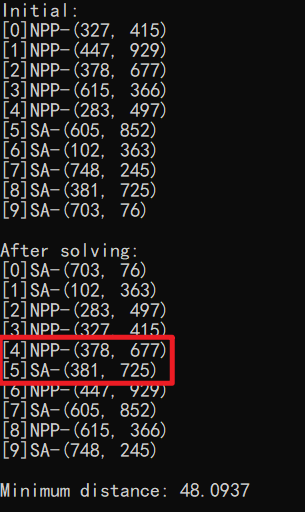
\includegraphics[scale=0.8]{images/run1.png}\;\;\;\;\;
        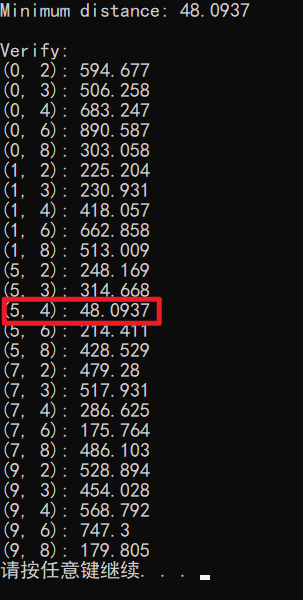
\includegraphics[scale=0.7]{images/run2.png}
    \end{figure}

\end{sloppypar}
\end{document}
